\chapter{Verifica e Validazione}
\label{cap:verifica-validazione}
\section{Scopo del capitolo}
Questo capitolo descrive come è stata attuata la verifica e la validazione all'interno del progetto. Grazie al processo di verifica garantiamo che ogni attività dei processi svolti non introduca errori nel prodotto e che soddisfi i requisiti. Mentre con il processo di validazione viene determinato in maniera oggettiva che il prodotto sia conforme ai requisiti richiesti.
\section{Processo di verifica}
Durante tutto il periodo di tirocinio, ad ogni avanzamento di funzionalità e quindi cambio di requisito da soddisfare, con il tutor Antonio Fasolato è stato verificato che il codice sviluppato fino a quel momento fosse conforme con quanto aspettato e producesse output veritieri. Questo era aiutato inoltre dai controlli, inseriti nel codice, di validazione effettuati nei vari Controller e ulteriori controlli inseriti nei Service per garantire l’utilizzo di valori corretti.\\
Veniva effettuata dapprima un’analisi statica sul codice prodotto, eseguendo una lettura mirata focalizzandoci sugli errori più noti e probabili, andando verso errori più specifici in base alla funzionalità implementata.\\
Il software poi veniva eseguito per essere conforme alle attese e in caso di errori veniva eseguita un’ulteriore verifica successivamente alla mia correzione dell’errore presentatosi.\\
Svolgendo questa analisi regolarmente, permetteva di identificare e correggere errori evitando la loro propagazione nel corso della codifica.

\section{Testing}
Per garantire la sicurezza e l’affidabilità, negli ultimi giorni di tirocinio, sono stati introdotti i test di unità.\\
Questo processo è iniziato con lo studio delle seguenti tecnologie:
\begin{itemize}
\item JUnit, framework di testing per Java utilizzato per la scrittura e l’esecuzione di test d’unità. L’adozione delle annotazioni e dei vari metodi che fornisce semplica il processo di scrittura di questi test;
\item Mockito, framework di testing per Java che si concentra sulla creazione di oggetti simulati (mock) per testare unità di codice. Gli oggetti mock imitano il comportamento di oggetti reali, consentendo ai test di focalizzarsi su parti specifiche del codice, permettendo ai test di non dover interagire con database o sistemi esterni.
\end{itemize}

\subsection{Unit testing}
Tramite i due framework poco fa citati, è stato possibile introdurre i test di unità.\\
Gli unit test (test di unità) verificano il funzionamento corretto di singole unità di codice, come metodi o classi. Questi test vengono sviluppati isolandosi dalle dipendenze esterne permettendo di verificare che il codice funzioni correttamente e che produca risultati attesi.\\
Si è andato a testare ciò che valeva la pena testare, quindi ciò che io avevo prodotto come metodi o classi. Componenti introdotti da librerie o framework non hanno necessitato di test, dando per assodato il loro funzionamento.\\
Dato il poco tempo rimanente, per mettere in pratica quanto appreso, si è deciso di limitare lo svolgimento dei test su un \textit{@Service} semplice, \texttt{MilestoneService},andando a testare il corretto funzionamento dei suoi metodi.

\subsection{Esempio di un test effettuato}
\begin{figure}[H] 
    \centering 
    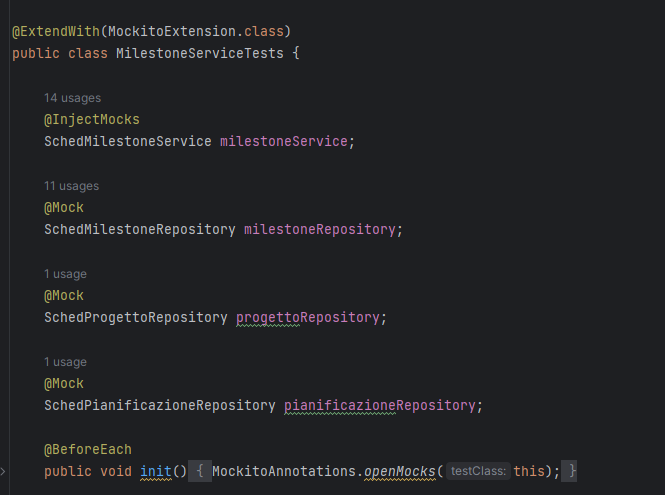
\includegraphics[width=0.85\columnwidth]{config-test} 
    \caption{Configurazione ambiente di testing}
\end{figure}
Per poter eseguire dei test su oggetti simulati (mock) , sono stati utilizzate le seguenti componenti.\\
Tramite l'annotazione \textit{@Mock} sono stati creati i componenti mock da iniettare all’interno del Service sotto test tramite l’annotazione \textit{@InjectMocks}. Tramite il metodo \texttt{init()}, annotato con \textit{@BeforeEach}, inizializziamo i metodi che vogliamo mockare permettendo l’utilizzo delle annotazioni che Mockito fornisce.\\
Qui riporto un code snippet dei controlli eseguiti nel test inerente al metodo di creazione di una nuova Milestone. Per garantire il corretto funzionamento della creazione della Milestone, è stata testata ogni parte delicata che avrebbe compromesso il funzionamento del metodo ,controllando l’eccezione sollevata, al momento dell’errore, assicurando che fosse quella corretta.\\

\begin{figure}[H] 
    \centering 
    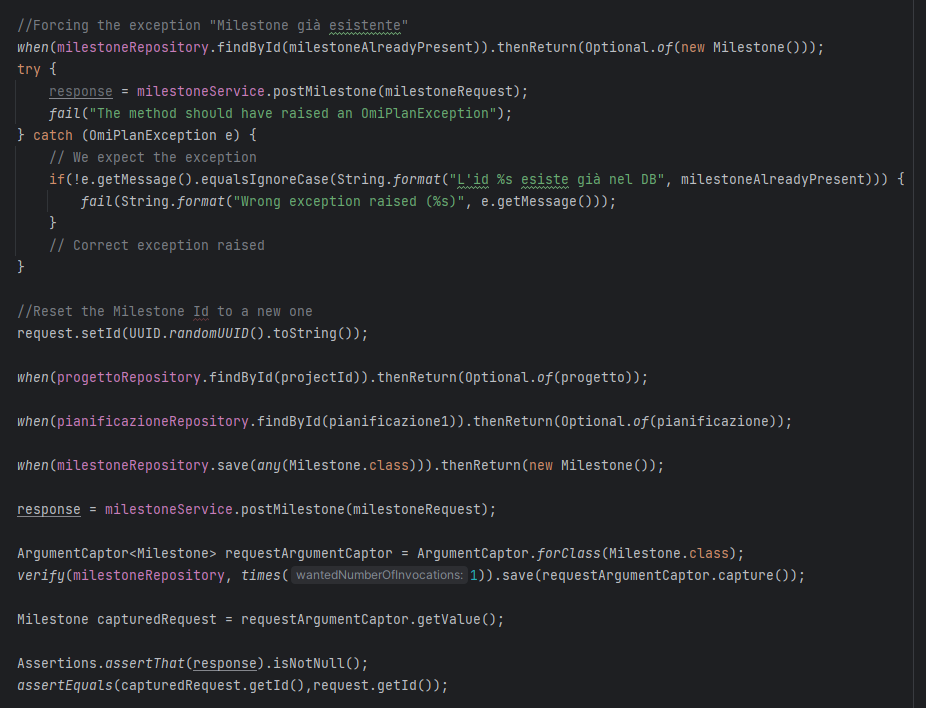
\includegraphics[width=0.9\columnwidth]{snippet-saveMilestone} 
    \caption{Code snippet test di creazione di una nuova Milestone}
\end{figure}

\noindent In questo snippet possiamo osservare come è stata forzata il lancio dell’eccezione quando si va a creare una Milestone con Id già esistente, controllando che sia stata proprio quella l’eccezione lanciata dal metodo. Mockito fornisce metodi che permettono lo stubbing\textsubscript{g} di metodi simulati come \texttt{when()}, che permette di assegnare un comportamento a metodi quando vengono chiamati, restituendo risultati specifici invece che eseguire codice reale. Con l’ausilio di questi metodi è stato possibile simulare la corretta creazione di una Milestone, verificando alla fine tramite \texttt{verify()} che il metodo \texttt{save()} della repository della Milestone venga chiamato una sola volta e che venga catturato, tramite un \texttt{ArgumentCaptor<>} (che permette di raccogliere i parametri passati in una funzione), la Milestone salvata col metodo \texttt{save()}.\\
Per accertare che questa parte di test abbia avuto successo, è stato verificato che la response ricevuta dal metodo non sia vuota e, dato che il DTO restituito differisce per molte caratteristiche dall’istanza completa di una Milestone, è stato ritenuto esaustivo garantire l’uguaglianza dei due Id. Queste verifiche sono state effettuate tramite metodi di asserzione forniti da JUnit.

\section{Validazione}
